
\documentclass[11pt]{article}
\usepackage[%
  papersize={12.8cm,9.6cm},
  hmargin=1cm,%
  vmargin=1cm,%
  head=0.4cm,% might be changed later
  headsep=0pt,%
  foot=0.5cm% might be changed later
]{geometry}% http://ctan.org/pkg/geometry

\RequirePackage{amsmath}
\RequirePackage{amssymb}
\RequirePackage{amsthm}
%\RequirePackage{algorithmic}
%\RequirePackage{algorithm}
%\RequirePackage{theorem}
%\RequirePackage{eucal}
\RequirePackage{color}
\RequirePackage{url}
\RequirePackage{mdwlist}

\RequirePackage[all]{xy}
\CompileMatrices
\RequirePackage{hyperref}
\RequirePackage{graphicx}
\RequirePackage{relsize}

\usepackage{setspace}


\renewcommand{\baselinestretch}{1.3} 

% xelatex:
\usepackage{fontspec}
\defaultfontfeatures{Ligatures=TeX}
%\usepackage[small,sf,bf]{titlesec}
%\setromanfont{DejaVu Serif}
%\setromanfont{Droid Serif}
%\setromanfont{Gentium} % nice! a bit fluffy
\setromanfont{Gentium Book Basic} % more bold

%\linespread{1.5}
%\linespread{1.4}

\RequirePackage{graphicx}
\usepackage{color}
\usepackage{amsfonts}


%\def\heading #1{\vskip 20pt \noindent\underline{\large \bf #1}\vskip 5pt}
\def\heading #1{\centerline{\underline{\bf\LARGE #1}}}
%\def\vsp {\vskip 0.5cm}
\def\vsp {\vspace*{0.5cm}}
\def\hsp {\ \ \ \ }
\def\half {\frac{1}{2}}

\def\ket #1{|#1\rangle}
\def\bra #1{\langle #1|}
\newcommand{\braket}[2]{\langle{#1}|{#2}\rangle}
%\def\point {\vskip 5pt $\to$\ \ }
%\def\point {\vskip 5pt $\Longrightarrow$\ \ }
%\def\point {\vskip 5pt $\bigodot$\ \ }
\def\point {\vskip 5pt $\hookrightarrow$\ \ }
\def\Tr{\mbox{Tr}}

\begin{document}

\large

\pagenumbering{gobble}

%%%%%%%%%%%%%%%%%%%%%%%%%%%%%%%%%%%%%%%%%%%%%%%%%%%%%%%%%%%


\vspace*{1.0cm}
\centerline{\LARGE Numerically Probing }
\vsp
\centerline{\LARGE The Gauge Color Code Hamiltonian}
\vspace{1.0cm}

\centerline{\Large Simon Burton}

\vsp

\centerline{November 2018}

\vsp
%\centerline{simon@arrowtheory.com}

\newpage %%%%%%%%%%%%%%%%%%%%%%%%%%%%%%%%%%%%%%%%%%%%%%%%%%%%%%%%%%%

%\heading{A Double Life}

\vspace*{-1.0cm}
{\centerline{\underline{\bf A Double Life}}}
\vspace*{-0.0cm}
\begin{center}
\resizebox{10cm}{!} {
\begin{tabular}{|ccc|}
\hline
Code       &  & Hamiltonian \\
\hline
$G$        &  $ \longleftrightarrow$ & $H = \sum_{g\in G} g $ \\
error & $\longleftrightarrow$ & excitations \\
\hline
stabilizer code & $\longleftrightarrow$ & frustration free \\
 & & spectral gap = 2 \\
\hline
subsystem code & $\longleftrightarrow$ &  frustrated \\
 & & spectral gap = ?? \\
\hline
\end{tabular}}
\end{center}

% XXX mention CSS -> stoquastic XXX


\newpage %%%%%%%%%%%%%%%%%%%%%%%%%%%%%%%%%%%%%%%%%%%%%%%%%%%%%%%%%%%

%\heading{A Double Life}

\vspace*{-1.0cm}
{\centerline{\underline{\bf A Double Life}}}
\vspace*{-0.0cm}
\begin{center}
\begin{tabular}{|ccc|}
\hline
Code       & & Hamiltonian \\
$G$        & $ \longleftrightarrow $ & $H = \sum_{g\in G} g $ \\
\hline
4D toric code       &            &  \\
stabilizer code & $\longleftrightarrow$ & commuting \\
single-shot error correction & $\longleftrightarrow$   &  energy barrier \\
 & & spectral gap = 2 \\
 & & quantum memory \\
\hline
3D gauge color code &            &  \\
subsystem code & $\longleftrightarrow$ &  frustrated \\
single-shot error correction &  $\longleftrightarrow$  &  quantum memory?? \\
 & & spectral gap = ?? \\
\hline
\end{tabular}
\end{center}

% XXX mention CSS -> stoquastic XXX

\newpage %%%%%%%%%%%%%%%%%%%%%%%%%%%%%%%%%%%%%%%%%%%%%%%%%%%%%%%%%%%

%\heading{A Double Life}
%{\centerline{\underline{\bf A Double Life}}}

\vspace*{-1.0cm}
{\centerline{\underline{\bf A Double Life}}}
\begin{center}
\resizebox{10cm}{!} {
\begin{tabular}{|ccc|}
\hline
Code       & & Hamiltonian \\
$G$        & $ \longleftrightarrow $ & $H = \sum_{g\in G} g $ \\
\hline
2D Bacon-Shor  & $\longleftrightarrow$ & 2D compass \\
subsystem code & $\longleftrightarrow$ &  frustrated \\
extensive stabilizers & $\longleftrightarrow$   &  gapless \\
\hline
3D gauge color code &            &  \\
subsystem code & $\longleftrightarrow$ &  frustrated \\
bounded stabilizers & $\longleftrightarrow$   &  gapped??? \\
\hline
\end{tabular}}
\end{center}

\newpage %%%%%%%%%%%%%%%%%%%%%%%%%%%%%%%%%%%%%%%%%%%%%%%%%%%%%%%%%%%

\heading{Conjecture}


\vsp
\centerline{
bounded stabilizer generators $\Rightarrow$
gapped Hamiltonian}
\vsp
\centerline{\LARGE ???}

%\vsp
%Compare: 
%
%\centerline{
%pointlike excitations $\Leftrightarrow$
%topological order}

\newpage %%%%%%%%%%%%%%%%%%%%%%%%%%%%%%%%%%%%%%%%%%%%%%%%%%%%%%%%%%%

\heading{Conjecture}
Unbounded stabilizer generators $\Rightarrow$
gapless Hamiltonian.
Intuition from double-well potential:
$$
    H = 2\ket{1}\bra{1}
    + \ket{1}\bra{2} 
    + \ket{2}\bra{1} 
    + ...
    + 2\ket{n}\bra{n}.
$$
\vsp
\centerline{
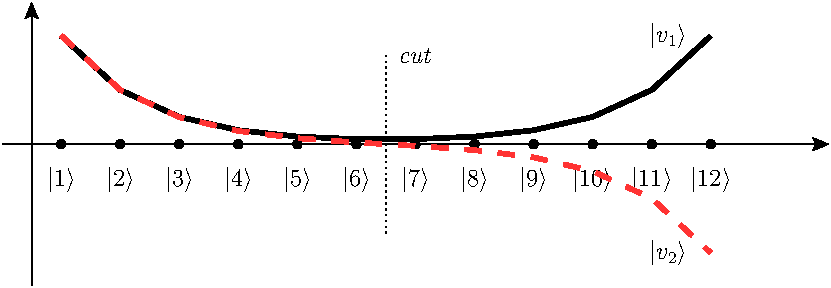
\includegraphics[width=0.8\textwidth]{pic-dwell.pdf}}
\vspace*{-1.0cm}
Gapless Hamiltonian as $n\to \infty.$


\newpage %%%%%%%%%%%%%%%%%%%%%%%%%%%%%%%%%%%%%%%%%%%%%%%%%%%%%%%%%%%

\heading{CSS Subsystem Code Hamiltonians}


When the subsystem gauge operators separate into
$X$ and $Z$ type operators,
$$
    G = G_X \cup G_Z
$$
these give rise to momentum and potential energy terms
in the Hamiltonian:
\vspace*{-0.5cm}
$$
H(G_X, G_Z) = \sum_{g\in G_X} g + \sum_{g\in G_Z} g  =  U_X + V_Z.
$$
Block diagonalized by stabilizer eigenvalues:
\vspace*{-0.4cm}
$$
    H = \bigoplus_{\{\lambda \}} H_{\{\lambda\}}
$$


\newpage %%%%%%%%%%%%%%%%%%%%%%%%%%%%%%%%%%%%%%%%%%%%%%%%%%%%%%%%%%%

\heading{3D Gauge Color Code}

\vsp
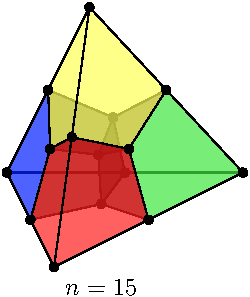
\includegraphics[width=0.3\textwidth]{pic-gcolor-1.pdf}

$X/Z$ gauge operators live on the 2D faces

$X/Z$ stabilizers live on the 3D cells

\rightline{[Bombin2015]}

\newpage %%%%%%%%%%%%%%%%%%%%%%%%%%%%%%%%%%%%%%%%%%%%%%%%%%%%%%%%%%%

\heading{3D Gauge Color Code}

\vsp
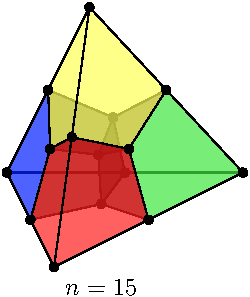
\includegraphics[width=0.2\textwidth]{pic-gcolor-1.pdf}
\hsp
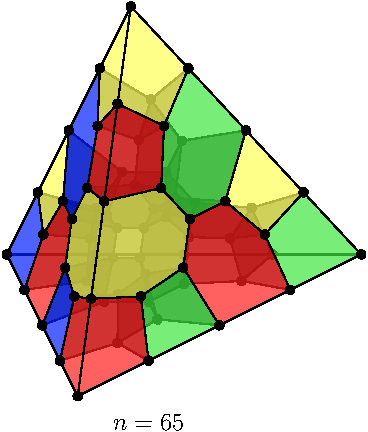
\includegraphics[width=0.3\textwidth]{pic-gcolor-2.pdf}
\hsp
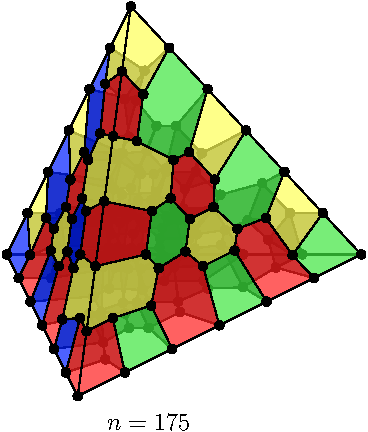
\includegraphics[width=0.4\textwidth]{pic-gcolor-3.pdf}

\rightline{[Bombin2015]}


%\newpage %%%%%%%%%%%%%%%%%%%%%%%%%%%%%%%%%%%%%%%%%%%%%%%%%%%%%%%%%%%
%
%\heading{3D Gauge Color Code}
%
%\vsp
%Hamiltonian is a sum of 6 mutually commuting pieces.
%
%\vsp
%Hamiltonian is block diagonalized by stabilizers.

\newpage %%%%%%%%%%%%%%%%%%%%%%%%%%%%%%%%%%%%%%%%%%%%%%%%%%%%%%%%%%%

\heading{3D Gauge Color Code}

\vsp 
Hamiltonian is a sum of $6$ mutually commuting pieces.

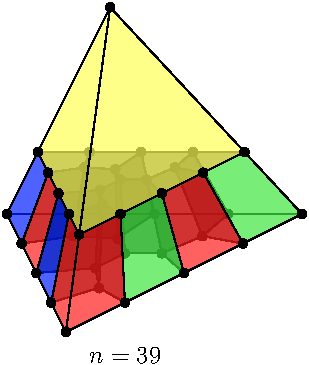
\includegraphics[width=0.4\textwidth]{pic-gcolor-15.pdf}
\hsp\hsp
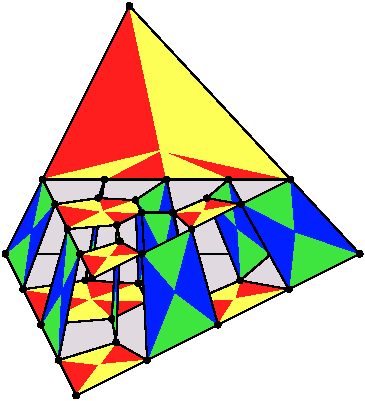
\includegraphics[width=0.4\textwidth]{pic-gcolor-ideal.pdf}

\rightline{[Burton2018]}

\newpage %%%%%%%%%%%%%%%%%%%%%%%%%%%%%%%%%%%%%%%%%%%%%%%%%%%%%%%%%%%

\heading{The Spectral Gap}

Exact diagonalization results
\begin{center}
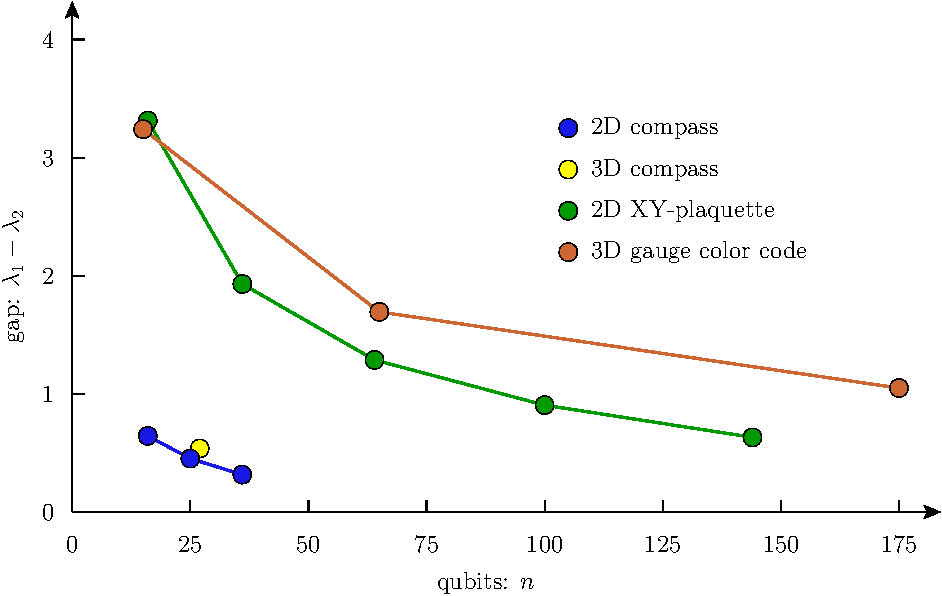
\includegraphics[width=0.8\textwidth]{pic-gap.pdf}
\end{center}

\vspace*{-0.4cm}
\rightline{[Burton2018]}

\newpage %%%%%%%%%%%%%%%%%%%%%%%%%%%%%%%%%%%%%%%%%%%%%%%%%%%%%%%%%%%

\heading{3D Gauge Color Code}

%Exact diagonalization results: Hamiltonian blocks
The weight of the frustrated stabilizer:
$w(S_Z).$

\begin{center}
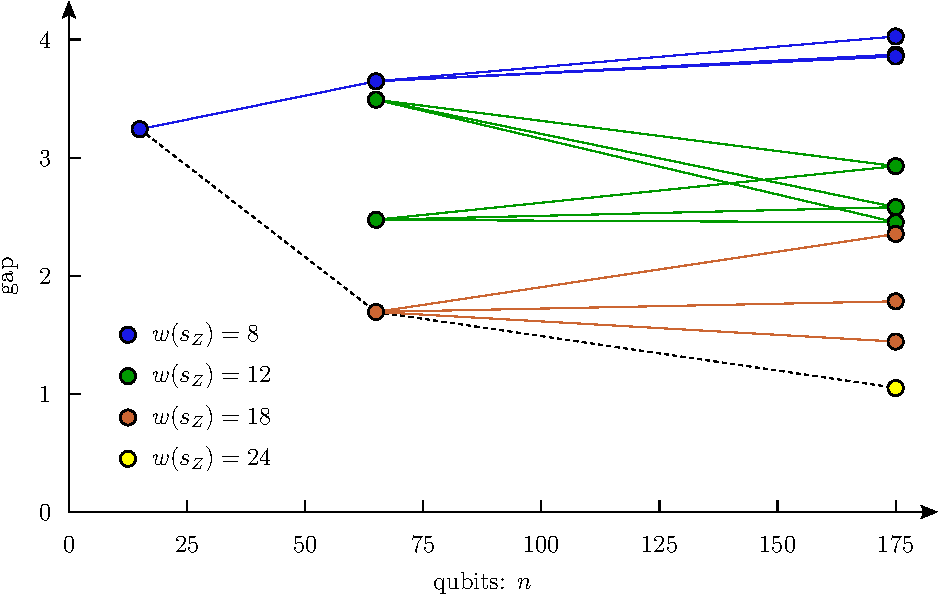
\includegraphics[width=0.8\textwidth]{pic-gap-stabs.pdf}
\end{center}

\vspace*{-0.4cm}
\rightline{[Burton2018]}
%arXiv:1801.03243

\newpage %%%%%%%%%%%%%%%%%%%%%%%%%%%%%%%%%%%%%%%%%%%%%%%%%%%%%%%%%%%

\heading{Quantum Monte-Carlo}

\vsp
Finite temperature partition function:
\begin{align*}
    Z =\ &\Tr( e^{\beta H} ) \\
      =\ &\Tr\bigl( I + \beta H 
        + \frac{1}{2} \beta^2 H^2
        + \frac{1}{3!} \beta^3 H^3
        + ... \bigr) \\
    =\ &\ \  \sum_{\sigma_0} \braket{\sigma_0}{\sigma_0} 
       + \beta \sum_{\sigma_0} \bra{\sigma_0} H \ket{\sigma_0} \\
     &  + \frac{1}{2} \beta^2 
        \sum_{\sigma_0, \sigma_1} \bra{\sigma_0} H \ket{\sigma_1}
        \bra{\sigma_1} H \ket{\sigma_0} \\
     &  + \frac{1}{3!} \beta^3 
        \sum_{\sigma_0, \sigma_1, \sigma_2}
        \bra{\sigma_0} H \ket{\sigma_1}
        \bra{\sigma_1} H \ket{\sigma_2}
        \bra{\sigma_2} H \ket{\sigma_0} + ...\\
\end{align*}

\newpage %%%%%%%%%%%%%%%%%%%%%%%%%%%%%%%%%%%%%%%%%%%%%%%%%%%%%%%%%%%

\heading{Quantum Monte-Carlo}

%$$
%    \langle H \rangle = \frac{d}{d\beta} \ln Z 
%    = \frac{1}{Z} \frac{dZ}{d\beta}
%$$

\begin{align*}
    Z &= \sum_{n=0}^{\infty} \frac{\beta^n}{n!}
        \sum_{\{\sigma_i\}} 
            \bra{\sigma_0} H \ket{\sigma_1} ...
            \bra{\sigma_{n-1}} H \ket{\sigma_0} \\
    \langle H \rangle &= \frac{1}{Z} 
        \sum_{n=0}^{\infty} \frac{\beta^n}{n!}
        \sum_{\{\sigma_i\}} 
            \bra{\sigma_0} H \ket{\sigma_1} ...
            \bra{\sigma_{n+1}} H \ket{\sigma_0} \\
        &= \frac{1}{Z} 
        \sum_{n=1}^{\infty} \frac{\beta^n}{n!}
        \frac{n}{\beta}
        \sum_{\{\sigma_i\}} 
            \bra{\sigma_0} H \ket{\sigma_1} ...
            \bra{\sigma_{n}} H \ket{\sigma_0} \\
        &= \frac{\langle n \rangle}{\beta}
\end{align*}
\vspace*{-0.4cm}
Stochastic series expansion [Sandvik2003].

\newpage %%%%%%%%%%%%%%%%%%%%%%%%%%%%%%%%%%%%%%%%%%%%%%%%%%%%%%%%%%%

\heading{Metropolis Algorithm}

Markov chain random jumps:
\begin{align*}
    &\bra{\sigma_0} H \ket{\sigma_1} ...  \bra{\sigma_{n}} H \ket{\sigma_0} \\
\longrightarrow &\\
    &\bra{\sigma'_0} H \ket{\sigma'_1} ...  \bra{\sigma'_{n'}} H \ket{\sigma'_0} 
\end{align*}
%
%\newpage %%%%%%%%%%%%%%%%%%%%%%%%%%%%%%%%%%%%%%%%%%%%%%%%%%%%%%%%%%%
%
%\heading{Metropolis Algorithm}
%
Random walk over words,
$$ g_1,...,g_n \in G_X,\ \ \mbox{such that}\ \ \ g_1...g_n = 1, $$
and the initial spin configuration: $\ket{\sigma_0}.$

\newpage %%%%%%%%%%%%%%%%%%%%%%%%%%%%%%%%%%%%%%%%%%%%%%%%%%%%%%%%%%%

\heading{Metropolis Algorithm}

\vsp
Random walk over words,
$$ g_1,...,g_n \in G_X,\ \ \mbox{such that}\ \ \ g_1...g_n = 1. $$

$g_1...g_n$ is a product of {\it relators:}
$$
    1,\  gg,\  ghg^{-1}h^{-1}
$$
and words built from $\mbox{Ker}(G_X^\top).$


\newpage %%%%%%%%%%%%%%%%%%%%%%%%%%%%%%%%%%%%%%%%%%%%%%%%%%%%%%%%%%%

\heading{Jump Operations}

\vsp
1) Insert identity

\begin{align*}
&... \bra{\sigma_{i-1}} H \ket{\sigma_i}\bra{\sigma_{i}} H \ket{\sigma_{i+1}}... \\
\longrightarrow &\\
&... \bra{\sigma_{i-1}} H \ket{\sigma_i}
    \bra{\sigma_{i}} H \ket{\sigma_{i}} 
    \bra{\sigma_{i}} H \ket{\sigma_{i+1}}... \\
\end{align*}


\newpage %%%%%%%%%%%%%%%%%%%%%%%%%%%%%%%%%%%%%%%%%%%%%%%%%%%%%%%%%%%

\heading{Jump Operations}

\vsp
2) Remove identity

\begin{align*}
&... \bra{\sigma_{i-1}} H \ket{\sigma_i}
    \bra{\sigma_{i}} H \ket{\sigma_{i}} 
    \bra{\sigma_{i}} H \ket{\sigma_{i+1}}... \\
\longrightarrow &\\
&... \bra{\sigma_{i-1}} H \ket{\sigma_i}\bra{\sigma_{i}} H \ket{\sigma_{i+1}}... \\
\end{align*}

\newpage %%%%%%%%%%%%%%%%%%%%%%%%%%%%%%%%%%%%%%%%%%%%%%%%%%%%%%%%%%%

\heading{Jump Operations}

\vsp
3) Replace a pair

\begin{align*}
&... \bra{\sigma_{i-1}} H \ket{\sigma_i}
    \bra{\sigma_{i}} H \ket{\sigma_{i-1}} ...\\
\longrightarrow &\\
&... \bra{\sigma_{i-1}} H \ket{\sigma'_i}
    \bra{\sigma'_{i}} H \ket{\sigma_{i-1}} ...\\
\end{align*}


\newpage %%%%%%%%%%%%%%%%%%%%%%%%%%%%%%%%%%%%%%%%%%%%%%%%%%%%%%%%%%%

\heading{Jump Operations}

\vsp
4) swap

\vsp
For $g, h \in G_X:$

\begin{align*}
&... \bra{\sigma} H \ket{\sigma + g}
    \bra{\sigma + g} H \ket{\sigma+g+h}... \\
\longrightarrow &\\
&... \bra{\sigma} H \ket{\sigma + h}
    \bra{\sigma + h} H \ket{\sigma+h+g}... \\
\end{align*}


\newpage %%%%%%%%%%%%%%%%%%%%%%%%%%%%%%%%%%%%%%%%%%%%%%%%%%%%%%%%%%%

\heading{Jump Operations}

\vsp
5) flip a spin

\begin{align*}
    \bra{\sigma_0} \longrightarrow  \bra{\sigma_0 + k} 
\end{align*}

where $k = (...0, 0, 1, 0, 0...)$.

\newpage %%%%%%%%%%%%%%%%%%%%%%%%%%%%%%%%%%%%%%%%%%%%%%%%%%%%%%%%%%%

\heading{Convergence}

\vsp
\underline{Theorem.}
Given a CSS subsystem code Hamiltonian
$$H(G_X, G_Z) = U_X + V_Z$$
the above Markov chain converges to the partition
function distribution iff $\mbox{Ker}(G_X^\top)$ is trivial.

\vsp
\underline{Proof:}
The Markov chain is
connected iff $\mbox{Ker}(G_X^\top)$ is trivial.

\end{document} %%%%%%%%%%%%%%%%%%%%%%%%%%%%%%%%%%%%%%%%%%%%%%%%%%%%%%%%%%%

